%%%%%%%%%%%%%%%%%%%%%%%%%%%%%%%%%%%%%%%%%%%%%%%%%%%%%%%%%%%%%%%%%%%%%%%%%%%%%%%%%%%%
%%----------------------------------------------------------------------------------
% DO NOT Change this is the required setting A4 page, 11pt, oneside print, book style
%%----------------------------------------------------------------------------------
\documentclass[a4paper,11pt,oneside]{book}
\usepackage{CS_report} 
%%%%%%%%%%%%%%%%%%%%%%%%%%%%%%%%%%%%%%%%%%%%%%%%%%%%%%%%%%%%%%%%%%%%%%%%%%%%%%%%%%%%

\begin{document}

    \captionsetup[figure]{margin=1.5cm,font=small,name={Figure},labelsep=colon}
    \captionsetup[table]{margin=1.5cm,font=small,name={Table},labelsep=colon}

    \frontmatter
    \pagenumbering{arabic} % Start counting at 1 immediately

    %%%%%%%%%%%%%%%%%%%%%%%%%%%%%%%%%%%%%%%%%%%%%%%%%%%%%%%%%%%%%%%%%%%%%%%%%%%%
    %% COVER PAGE — Forced to show Footer
    %%%%%%%%%%%%%%%%%%%%%%%%%%%%%%%%%%%%%%%%%%%%%%%%%%%%%%%%%%%%%%%%%%%%%%%%%%%%
    \begin{titlepage}
        \thispagestyle{fancy} % <--- THIS FORCES THE FOOTER ON THE COVER
        
        % Logo 
        \noindent
\includegraphics[width=5cm]{figures/logo_supcom.png}

        \vspace{0.2cm}
        \noindent\rule{\textwidth}{1.2pt}
        \vspace{0.4cm}

        \begin{center}
            {\large\textit{Telecommunications Engineering Degree Programme}}\\[0.1cm]
            {\large\textit{Option: Cyber Security and Defense (CySed)}}\\[0.8cm]

            {\fontsize{22}{28}\selectfont\textbf{Final Year Project Report}}\\[0.8cm]

            {\large\textit{Subject:}}\\[0.2cm]
            {\Large\guillemotleft\ Canny TMS\ \guillemotright}\\[0.8cm]

            {\large\textit{Prepared by:}}\\[0.2cm]
            {\Large Mohamed Ayoub Ben Omrane}\\[0.6cm]

            {\large\textit{Supervisors:}}\\[0.2cm]
            {\large Mr Mohamed-Bêcha Kaaniche}\\[0.1cm]
            {\large Mr Mourad Menif}\\[0.6cm]

            {\large\textit{Project proposed and carried out in collaboration with}}\\[0.2cm]
            %{\large\textcolor{black}{Canny Vision}}\\[0.3cm]
            \includesvg[width=2.5cm]{figures/logo_cannyvision}\\[0.5cm]

            {\large Academic year: 2025-2026}
        \end{center}

        \vfill 
        \begin{center}
            \setlength{\fboxsep}{0pt} 
            % 1. The Navy Top Border
            \colorbox{SupcomNavyBorder}{% 
                \parbox{\textwidth}{\rule{0pt}{3pt}} 
            }\\[-1pt] 
            % 2. The Light Blue Background Box
            \setlength{\fboxsep}{10pt}
            \colorbox{SupcomLightBlue}{%
                \parbox{\dimexpr\textwidth-2\fboxsep}{%
                    \centering\small\color{black} % Text should be black on light blue
                    Ecole Supérieure des Communications de Tunis\\[2pt]
                    \textbf{SUP'COM}\\[2pt]
                    \textit{2083 Cité Technologique des Communications -- Elghazala -- Ariana -- Tunisie}\\[2pt]
                    \textit{Tél. +216 70 240 900 \textendash\ site web : www.supcom.tn}
                }%
            }
        \end{center}
        % Note: The footer will appear BELOW this box because of \thispagestyle{fancy}
    \end{titlepage}

    % -------------------------------------------------------------------
    % Following Pages (Abstract, etc.)
    % -------------------------------------------------------------------
    % DO NOT reset pagenumbering here, so the next page naturally becomes Page 2
    
    \chapter*{Abstract}
\addcontentsline{toc}{chapter}{Abstract}

{\setstretch{1.2}
Canny Vision is a company specializing in computer vision solutions, whose
project teams require an efficient means of tracking tasks, managing goals, and resolving
technical issues across multiple concurrent projects. Existing commercial platforms such as
Jira or ClickUp were ruled out on two grounds: hosting sensitive project data on third-party
servers raises data-sovereignty and security concerns incompatible with the company's
zero-trust posture, and no off-the-shelf tool can be fully tailored to the company's specific
workflows and internal constraints.

This report presents \textbf{Canny TMS}, a custom-built Ticket Management System designed
and developed as an end-to-end internal solution for Canny Vision. The system integrates
seamlessly with the company's pre-existing Identity and Access Management infrastructure,
based on OAuth~2.1 with PKCE, ensuring that all authentication and authorization flows
remain under full organizational control. The frontend is implemented in pure vanilla
JavaScript using the company's in-house MVP rendering engine, with no reliance on
third-party libraries. A fine-grained Attribute-Based Access Control model, conformant
with the NIST SP~800-162 standard, enforces workspace-level authorization policies and
governs every protected operation within the system.

Canny TMS is fully operational and currently in production use across multiple teams at
Canny Vision. It supports the complete lifecycle of epics and tickets --- from creation
and assignment to status tracking and threaded commenting --- while maintaining strict
data isolation within a self-hosted deployment.

The system demonstrates how security-first design constraints and a zero-external-dependency
policy can be reconciled with a productive and user-friendly collaboration tool, and lays
the groundwork for future enhancements such as a Policy Administration Point and advanced
analytics dashboards.

\bigskip
\noindent\textbf{Keywords:} ticket management, zero-trust architecture, OAuth~2.1 with PKCE,
attribute-based access control, vanilla JavaScript.
}

    \chapter*{Foreword}
\addcontentsline{toc}{chapter}{Foreword}

This report presents the work carried out during my final year internship at \textbf{Canny Vision}, a company specialising in computer vision solutions. The internship ran from \textbf{16 February 2026 to 12 June 2026}, under the supervision of \textbf{Mr Mohamed-Bêcha Kaaniche} as external supervisor and \textbf{Mr Mourad Menif} as academic supervisor. The main focus of the project was to design and develop a Ticket Management System (TMS) tailored to the specific operational and security needs of Canny Vision's teams.

\bigskip

It is with sincere appreciation that I dedicate these lines to everyone who contributed, directly or indirectly, to the completion of this work.

I would like to express my gratitude to Mr~Kaaniche for his guidance, availability, and constructive feedback throughout the project. His support at every stage of development was genuinely valuable.

I would also like to thank Mr~Menif for his advice and academic perspective, which helped me maintain a clear view of the broader context of the work.

My thanks go to \textbf{SUP'COM} for the academic foundation it provided and for the opportunity to apply engineering principles in a real professional environment.

Finally, I extend my appreciation to the jury members who will take the time to read and evaluate this report.

\bigskip\bigskip

\noindent\textbf{Responsible AI Use Declaration.}
Generative AI tools (Claude) were used during the preparation of this report for language improvement, LaTeX formatting, and structuring certain sections. All technical content, design decisions, implementation work, and analysis are entirely my own. The report faithfully reflects my understanding and the work I carried out during the internship.


    \tableofcontents
    \listoffigures
    \listoftables

    \chapter*{Glossary and Abbreviations}
\addcontentsline{toc}{chapter}{Glossary and Abbreviations}

\begin{abbrv}
	\item[API] Application Programming Interface
	\item[CRUD] Create, Read, Update, Delete
	\item[IAM] Identity and Access Management
	\item[JWT] JSON Web Token
	\item[PFE] Projet de Fin d'Etudes
\end{abbrv}

    \chapter*{General Introduction}
\addcontentsline{toc}{chapter}{General Introduction}

\section*{Context and Application Domain}
This project was carried out at \textbf{Canny Vision}, a startup that specializes in computer vision solutions. The company provides a wide range of AI services, including shoplifting detection, tracking traffic violations, and performing data analysis on retail customers—such as calculating the average time spent in specific aisles based on people entering and exiting the shop.

\section*{Problem Statement and Motivation}
For a company of this size and technical nature, it is mandatory to use a system that tracks progress, tickets, and business objectives. While there are many popular market solutions like Jira and ClickUp that offer great UI/UX design and numerous features, Canny Vision cannot tolerate storing its data on external servers. This represents a significant security issue and creates a risky reliance on third-party companies, which is unacceptable for a firm handling sensitive surveillance data.

\section*{Project Objectives and Expected Deliverables}
Because of these security concerns, I was assigned the responsibility of developing a custom \textbf{Ticket Management System (TMS)} tailored specifically to the company's needs. The primary objective was to deliver a secure platform built with a \textbf{Zero Trust architecture}, ensuring that all necessary security measures are handled internally to maintain absolute control over the data.

\section*{Summary of Work Completed}
During this internship, I developed the full system using a stack consisting of \textbf{Jakarta EE}, \textbf{WildFly} and \textbf{Vanilla JS}. The work involved designing the core architecture, implementing custom security interceptors for fine-grained access control, and building a responsive interface that meets the operational needs of the Canny Vision team. The application is also delivered as a \textbf{Progressive Web App}, meaning team members can consult their tickets and epics offline and receive push notifications when a ticket is assigned to them.

\section*{Chapter-by-Chapter Roadmap}
This report is organized into four main chapters as follows:
\begin{itemize}
    \item \textbf{Chapter 1: State of the Art} provides a review of existing solutions and the technical context of the project.
    \item \textbf{Chapter 2: Architecture and Conception} details the design phase and the proposed technical solution.
    \item \textbf{Chapter 3: Environment and Realisation} describes the tools used and the actual implementation phase of the system.
    \item \textbf{Chapter 4: Analysis, Tests, and Performance Evaluation} presents the testing results and an evaluation of the system's efficiency.
\end{itemize}

Finally, the report ends with a \textbf{Conclusion} summarizing the results of the internship and potential future improvements.

    \mainmatter 
    % Note: \mainmatter usually resets page numbers to 1. 
    % If you want continuous numbering (Cover=1, Intro=7, etc.), 
    % comment out \mainmatter or use \pagenumbering{arabic} again after it.

    \chapter{State of the Art}

\section{Introduction}

A Ticket Management System is at its core a collaboration tool: it lets teams track work items, link them to higher-level goals, and know at a glance who is doing what and where things stand. For a technical company like Canny Vision, which builds computer vision products involving sensitive surveillance data, such a system is not optional—it is how the team coordinates internally on every project.

The question is not whether to use one, but which one. This chapter surveys the existing solutions, examines the access control standards that govern how such systems enforce permissions, and reviews the technology choices made for the backend and the frontend—leading to the justification of the stack selected for this project.

%% ─────────────────────────────────────────────────────────────────────────────
\section{Existing Ticket Management Solutions}

\subsection{Commercial SaaS Products}

The dominant players in the space—Jira, ClickUp, Asana, and Linear—are all Software-as-a-Service platforms. They store data on the vendor's infrastructure, which by design means the company has no control over where that data physically lives.

\textbf{Jira} (Atlassian) is the de facto standard in software teams. It offers a rich feature set: sprints, epics, custom workflows, automations, and deep integrations with CI/CD pipelines. Its complexity is well-documented; configuring a project correctly requires a non-trivial amount of administrator time, and the free tier imposes strict limits on users and storage.

\textbf{ClickUp} markets itself as an all-in-one replacement for every productivity tool. It covers task boards, docs, goals, time tracking, and dashboards. The breadth of features is impressive but introduces cognitive overhead for teams that only need the ticket-tracking subset.

\textbf{Linear} is the most developer-oriented of the group. It prioritises speed and keyboard-driven workflows, and its data model is simpler than Jira's. It is popular in startups that find Jira too heavy.

\textbf{Trello} takes a minimalist card-and-column approach (Kanban only) and is easy to onboard. It does not support epics or structured hierarchies by default, which makes it unsuitable for projects that need to link low-level tickets to business objectives.

The common limitation of all four tools is data residency. None of them can guarantee that company data stays within a specific jurisdiction or server, and the company is subject to the vendor's security posture, breach notifications, and data retention policies. For Canny Vision, which processes video feeds from physical premises and stores analysis results, storing work items on an external SaaS platform creates an unacceptable dependency.

\subsection{Self-Hosted Open-Source Alternatives}

Self-hosted systems address the data sovereignty issue but introduce a maintenance burden.

\textbf{Plane} is an open-source alternative to Linear, released in 2022. It supports issues, cycles (equivalent to sprints), modules (collections of issues), and custom states. It requires a Docker stack to run, and as of its early releases, lacked fine-grained workspace-level permission control.

\textbf{GitLab Issues} solves the problem for teams already on GitLab: issues, epics, milestones, and boards are built in. The drawback is that it tightly couples project management with code hosting. A company that does not want all team members in the git repository cannot cleanly separate the two concerns.

\textbf{Redmine} is a mature Rails-based project management tool with a long track record. Its permission model is role-based and reasonably expressive, but its interface shows its age. Plugin quality is inconsistent, and the setup for multi-tenant access control requires custom development anyway.

\textbf{Taiga} offers a clean Kanban/Scrum interface with epics and user stories. Like Plane, it needs its own infrastructure to self-host, and its access control model is relatively coarse.

\subsection{Summary and Gap}

\begin{table}[H]
    \centering
    \caption{Comparison of existing TMS solutions}
    \label{tab:tms-comparison}
    \renewcommand{\arraystretch}{1.3}
    \begin{tabular}{lcccc}
        \toprule
        \textbf{Solution} & \textbf{Data Sovereignty} & \textbf{Fine-Grained ACL} & \textbf{Epics + Tickets} & \textbf{Self-Hosted} \\
        \midrule
        Jira       & \texttimes & \checkmark & \checkmark & Partial (Data Center) \\
        ClickUp    & \texttimes & \checkmark & \checkmark & \texttimes \\
        Linear     & \texttimes & Limited    & \checkmark & \texttimes \\
        Plane      & \checkmark & Limited    & \checkmark & \checkmark \\
        GitLab     & \checkmark & \checkmark & \checkmark & \checkmark \\
        Redmine    & \checkmark & Limited    & Partial    & \checkmark \\
        \textbf{This project} & \checkmark & \checkmark & \checkmark & \checkmark \\
        \bottomrule
    \end{tabular}
\end{table}

None of the surveyed tools satisfies all three requirements simultaneously: full data control, a permission model fine-grained enough to express workspace-level roles, and a codebase the company can own and extend. This is the gap the current project addresses.

%% ─────────────────────────────────────────────────────────────────────────────
\section{Access Control Models}

Because the permission requirements of this system are non-trivial—two distinct role scopes that interact in specific ways—it is worth reviewing the main access control paradigms and understanding why a hybrid approach was chosen.

\subsection{Discretionary Access Control (DAC)}

DAC gives the resource owner the right to grant or revoke access to other users. Unix file permissions are the canonical example. This model is too loose for an organisation: a user could accidentally (or intentionally) share a resource with someone who should not have it.

\subsection{Role-Based Access Control (RBAC)}

RBAC assigns permissions to roles, and users are assigned to roles. The classic NIST RBAC model \cite{nist_rbac} defines four levels of increasing complexity: flat RBAC (users, roles, permissions), hierarchical RBAC (role inheritance), constrained RBAC (separation of duties), and symmetric RBAC.

RBAC works well when permissions map cleanly to job titles. In this system, the top-level business role—\texttt{ADMIN} or \texttt{MEMBER}—fits RBAC well: an admin has global permissions on workspaces and memberships regardless of context, and a member cannot act without being placed in a workspace first. This coarse-grained layer is issued by the IAM as a claim inside the JWT token.

The limitation of pure RBAC appears at the workspace level. Knowing that a user has the role \texttt{DEVELOPER} does not fully determine whether a given request is allowed—it also depends on whether the target ticket belongs to that developer, which workspace the ticket lives in, and whether the workspace is one the user is a member of. A static role cannot express that.

\subsection{Attribute-Based Access Control (ABAC)}

ABAC makes authorization decisions based on attributes of the subject (the user), the resource (the object being accessed), the action, and optionally the environment (time, IP, etc.) \cite{nist_abac}. Rules are written as policies that combine these attributes.

The ABAC model maps naturally to the workspace-level requirements: \textit{"a DEVELOPER can delete a ticket only if the ticket's owner is the requesting user"} is straightforwardly expressible as an attribute rule—\texttt{action == DELETE AND resource.owner == subject.username AND subject.workspace\_role == DEVELOPER}.

\subsection{The XACML Standard}

XACML (eXtensible Access Control Markup Language) is an OASIS standard \cite{xacml30} that formalises ABAC evaluation. Its architecture defines four components:

\begin{itemize}
    \item \textbf{PEP} (Policy Enforcement Point): intercepts the request and enforces the decision.
    \item \textbf{PDP} (Policy Decision Point): evaluates rules and returns a decision.
    \item \textbf{PIP} (Policy Information Point): retrieves missing attributes from external sources (database, LDAP, etc.).
    \item \textbf{PAP} (Policy Administration Point): manages and stores policy definitions.
\end{itemize}

The standard also specifies combining algorithms—how to aggregate multiple rule decisions into one final verdict. The two most security-relevant are \textit{deny-unless-permit} (deny by default, only grant if at least one rule explicitly allows) and \textit{permit-unless-deny} (the inverse).

This project does not implement XACML verbatim—the XML syntax and the full set of built-in functions are overkill for the scope. Instead, the authorization engine in the \texttt{core} module is \textit{inspired by} XACML: it has a PEP (a CDI interceptor bound to a custom \texttt{@RequireAuthorization} annotation), a PDP interface per tenant, a PIP interface for attribute enrichment, and a pluggable combining algorithm with \textit{deny-unless-permit} as the default. The design stays aligned with the standard's vocabulary while keeping the implementation lightweight.

\subsection{Zero Trust Architecture}

Zero Trust is a security model that rejects the idea of a trusted internal network. Every request must be authenticated and authorized regardless of where it originates \cite{nist_zerotrust}. The principle \textit{"never trust, always verify"} has concrete implications for implementation: no session sharing between services, short-lived tokens, explicit verification of identity on each request.

In practice, this means the system issues JWT tokens with a short expiry from the IAM module, and every API call to the TMS presents that token. The token is verified on each request without storing session state on the server—stateless authentication. The ABAC layer then makes a fresh decision on each call based on current resource attributes, not a cached permission snapshot.

%% ─────────────────────────────────────────────────────────────────────────────
\section{Technology Choices}

\subsection{Backend: Jakarta EE on WildFly}

The Java enterprise ecosystem in 2025 offers three serious contenders for a REST backend: Spring Boot, Quarkus, and Jakarta EE.

\textbf{Spring Boot} is the most widely used. It favours convention over configuration and builds quickly. The trade-off is that it is opinionated and pulls a large set of transitive dependencies. Critically for this project, Spring's interceptor and CDI equivalents work slightly differently from the Jakarta EE specifications—which matters when the authorization mechanism relies on \texttt{@InterceptorBinding} annotations that must behave precisely as the spec defines.

\textbf{Quarkus} is designed for cloud-native, GraalVM-native compilation, and fast startup times. It implements Jakarta EE APIs on top of its own Vert.x runtime. For a team building an internal system that runs on a managed server, the GraalVM compilation pipeline adds complexity without meaningful benefit.

\textbf{Jakarta EE on WildFly} is the standard enterprise Java specification implemented by a mature, battle-tested application server. WildFly implements the full Jakarta EE 10 profile—JAX-RS for REST endpoints, CDI for dependency injection, JPA with Hibernate for persistence, and the Interceptors specification for cross-cutting concerns. The authorization layer in this project depends directly on CDI's \texttt{Instance<T>} for tenant discovery and on the Interceptors spec for the PEP binding. Using the reference implementation guarantees predictable behavior.

\subsection{Frontend: Vanilla JavaScript with ESM Modules}

The frontend is a Single Page Application. The main architectural decision was whether to use a JavaScript framework (React, Vue, Angular) or to write vanilla JavaScript.

\textbf{React and Vue} are the dominant choices in 2025. They offer component models, reactive state management, and large ecosystems. The downside for this context is supply chain risk: a typical React project has hundreds of transitive npm dependencies, each of which is a potential attack surface. For a system handling sensitive internal data, minimising the dependency surface is not a secondary concern.

\textbf{Vanilla JavaScript with ES Modules} eliminates that risk. Modern browsers support native ES module imports, dynamic \texttt{import()}, and \texttt{import.meta}—there is no need for a bundler or a build step in development. The project uses Tailwind CSS via its standalone CLI (no Node.js dependency required at runtime) and \texttt{SortableJS} as the only runtime JavaScript dependency, for drag-and-drop on the Kanban board.

The architecture follows the \textbf{Model-View-Presenter} pattern. Each page module exports an \texttt{init} function that instantiates a Presenter, which coordinates a Model (responsible for API calls and reactive state via observables) and a View (responsible for DOM rendering and intent event emission). This separation makes each page independently testable and ensures that API-fetching logic is never mixed with DOM manipulation.

The application also ships a Service Worker implementing a layered caching strategy—navigation requests go network-first, static assets are cache-first—making the app usable in degraded network conditions.

%% ─────────────────────────────────────────────────────────────────────────────
\section{Chapter Conclusion}

The review of existing TMS products shows that no off-the-shelf tool satisfies the combination of data sovereignty, workspace-level fine-grained access control, and full ownership that Canny Vision requires. Self-hosted open-source alternatives come close on the data question but fall short on permission granularity.

The access control literature establishes that RBAC alone cannot express resource-ownership conditions. The ABAC model—formalised by XACML—provides the right vocabulary, and the Zero Trust principle supplies the security posture that governs how authentication and authorization interact at runtime.

On the technology side, Jakarta EE on WildFly was selected for its standards compliance and predictable CDI behaviour, while Vanilla JS with ES Modules was chosen to minimise the supply chain surface area and keep the frontend under full internal control.

The next chapter presents the architecture and design of the system built on these foundations.

    \chapter{Modeling and Design of the Proposed Solution}

\section{Introduction}
Introduce the proposed application and define its official name or brand.

\section{Requirements Analysis}
\begin{itemize}
    \item Functional requirements
    \item Non-functional requirements
    \item Constraints and assumptions
\end{itemize}

\section{Global Architecture}
Describe the high-level architecture and module decomposition (frontend, backend, data, IAM, etc.).

\begin{figure}[H]
    \centering
    % \includegraphics[width=0.9\textwidth]{figures/architecture-overview.png}
    \caption{High-level architecture of the proposed solution}
    \label{fig:architecture-overview}
\end{figure}

\section{Modeling}
Include relevant models and diagrams:
\begin{itemize}
    \item use case diagrams,
    \item class or domain model,
    \item sequence or activity diagrams,
    \item database model if applicable.
\end{itemize}

\section{Design Decisions}
Explain key decisions and trade-offs:
\begin{itemize}
    \item chosen frameworks and patterns,
    \item security and authorization choices,
    \item scalability and maintainability considerations.
\end{itemize}

\section{Chapter Conclusion}
Summarize how the design responds to identified requirements and prepares implementation.

// my own words that claude will use later to generate the actual content of the chapter.


./path means the root of the opened folder (rapport-pfe)

#introduction
Canny TMS, a custom-built Ticket Management System designed to meet the specific needs of Canny Vision, was my responsability
to design and develop.
#requirements analysis
## functional requirements
Canny vision already has its own internal identity access managment software that handles authenticatoin and authorizatoin
that's based on oauth2.1 with pkce (dear claude read ./middleware/iam module for more details and to understand how the iam works in detail)
so the app that I developed had to be compatible with the existing IAM and use it for all authentication and authorization needs.
Canny vision also don't use any frameworks or libraries for the frontend, so the app had to be developed using vanilla js and no external dependencies.
that's why they have their own developed mvp engine (youc can read ./frontend/scripts/mvp.js to understand how it works) that I had to use for the frontend development.
the app also had to be developed using a zero trust architecture, which means that all security measures had to be implemented internally and no data could be stored on external servers.
## non functional requirements
the ui/ux design had to be simple and intuitive, and the app had to be responsive and accessible on different devices.
the app also had to be scalable and maintainable, as it would be used by multiple teams
and would need to evolve over time to meet changing requirements.
#global architecture
I will pass a figure here later that shows the high level architecture of the system
 read it yourself and wrtie what you see fit
#modeling
same thing too for global architecute
#design decisions

bootstrap vs tailwindcss
I started with bootsrap , which is the company choice (imported from cdn ; doesn't expose secuirty issues)
it's good because blah blah but it limits the design and makes it look like every other bootstrap app, and it also has a lot of unused css that affects performance.
I convinced Mr Kaaniche to switch to tailwindcss, which is a utility-first css framework that allows for more flexibility and better performance.
In normal methods (not so secure app) it should be installed via npm and used as a build tool, but since we can't use any external dependencies, I used it with standalone cli where I isntalled the engine locally
read : https://tailwindcss.com/blog/standalone-cli  and put it in the report in its place(idk the actual page where we should put from wehre we got our information)


abac: 
nist standard : I spent time reading and analyzing the nist standard for access control : here's the link https://nvlpubs.nist.gov/nistpubs/specialpublications/nist.sp.800-162.pdf
integrate it too in the report
to actually implenet it I used authZforce whihc is an open source xacml engine where I donwloade the source code and inspired from to implmeent my own

[I will put here the figure of nist compliant abac]
and saying how I didn't implement PAP because it's too next leven and maybe later 

    \chapter{Environment and Implementation}

\section{Introduction}

Building a system from a blank repository is one thing; doing it inside an existing,
opinionated infrastructure is another. The first two weeks of the internship were spent
entirely on understanding what was already in place at Canny Vision before a single line
of project code was written. This chapter covers the environment that shaped the
implementation --- the tools chosen, the challenges encountered during setup, and the
phased progression from a working local environment to a deployed application.

\section{Development Environment}

\subsection{Migrating to Linux}

The workstation originally ran Windows. WildFly's management CLI relies on shell scripting
and file-permission semantics that translate poorly under WSL, and the Elytron-based TLS
configuration involves keytool commands that behave differently depending on which JDK is
on the \texttt{PATH}. Rather than fight the platform, the decision was made early on to
switch the operating system entirely to Linux. From that point, server management,
certificate handling, and Maven builds all worked predictably from a single terminal.

\subsection{WildFly: Not Your Everyday Application Server}

WildFly is not a server you configure with a handful of YAML files and restart in ten
seconds. Its domain model --- subsystems, socket bindings, security realms, deployment
descriptors, JNDI resources --- takes time to internalize. The official documentation is
thorough but assumes a baseline familiarity that takes a few days to build.

The payoff is significant, though. A single WildFly instance handles static file serving,
TLS termination, CORS policy enforcement, HSTS headers, database connection pooling via
JNDI, and WAR deployment --- all configured consistently through its CLI. For a
self-hosted setup, that consolidation is worth the upfront learning cost.

\subsection{Three Days and a Certificate}

The single most time-consuming obstacle during setup had nothing to do with application
code. After TLS was configured for the IAM module running at \texttt{iam.localhost}, the
frontend's fetch requests continued to fail with \texttt{SSLHandshakeException}, despite
the certificate appearing to be correctly installed.

The root cause, discovered after three days of logging and keytool inspection, was a
permissions mismatch. The \texttt{mkcert} command used to generate the local CA
certificate had been run with \texttt{sudo}. The resulting root certificate was installed
into the system truststore under the root user, and subsequently imported into the Oracle
JDK's \texttt{cacerts} file using \texttt{keytool} --- also under \texttt{sudo}. When
WildFly was later started as a normal user, the JVM resolved its cacerts from the
non-root user's environment, which had never seen the certificate. The two users' JDK
installations were pointing to different keystores.

The fix was straightforward once the cause was identified: regenerate the mkcert root CA
as the normal user and import it into the JDK cacerts that the application server actually
reads at runtime. The lesson was less about certificates and more about how JVM trust
resolution works in a multi-user Linux environment.

\section{Technology Stack}

\begin{table}[H]
    \centering
    \caption{Main technologies used in Canny TMS}
    \label{tab:techstack}
    \begin{tabular}{ll}
        \hline
        \textbf{Layer} & \textbf{Technology} \\
        \hline
        Application server   & WildFly 35 (Undertow, Elytron, JNDI)  \\
        Backend language     & Java 21 (Jakarta EE 11, MicroProfile Config 3.1) \\
        ORM                  & Hibernate 7 (JPA provider)            \\
        Build system         & Maven (multi-module POM)              \\
        Database             & MySQL                                 \\
        Frontend language    & Vanilla JavaScript (ES modules)       \\
        CSS framework        & Tailwind CSS (standalone CLI)         \\
        Local TLS            & mkcert + Oracle JDK keytool           \\
        Version control      & Git                                   \\
        IDE                  & IntelliJ IDEA                         \\
        \hline
    \end{tabular}
\end{table}

\section{Middleware Architecture: A Maven Multi-Module Project}

The backend is structured as a Maven multi-module project named \texttt{tms}, with three
child modules: \textbf{core}, \textbf{iam}, and \textbf{api}. The parent POM declares the
shared dependency versions and compiler settings (Java 21, Jakarta EE 11), while each
module's own POM declares only what is specific to it.

\begin{figure}[H]
    \centering
\begin{verbatim}
middleware/
├── pom.xml            (parent: tms)
├── core/              (JAR — shared utilities)
├── iam/               (WAR — authentication & token management)
└── api/               (WAR — business logic & REST endpoints)
\end{verbatim}
    \caption{Maven multi-module structure of the middleware}
    \label{fig:maven-structure}
\end{figure}

\subsection{The Core Module}

\texttt{core} is packaged as a JAR and is listed as a compile-time dependency of both
\texttt{iam} and \texttt{api}. It contains everything that the two application modules
need but that should not be duplicated: the ABAC framework abstractions
(\texttt{PolicyDecisionPoint}, \texttt{PolicyEnforcementPoint},
\texttt{PolicyInformationPoint} and their supporting model classes), the generic Jakarta EE
endpoint interfaces (\texttt{FetchableEndpoint}, \texttt{CreatableEndpoint}, etc.),
base entity classes (\texttt{AbstractEntity}, \texttt{RootEntity}), and shared utilities
such as the JSON object mapper and the authorization filter skeleton.

The HATEOAS support classes (\texttt{Resource}, \texttt{DTOResource}, and their collection
equivalents) also live in core, giving both modules a consistent way to wrap responses
with hypermedia links without repeating that logic.

\subsection{The IAM Module}

\texttt{iam} is deployed as a WAR under the context root \texttt{/rest-iam}. It was
already in place when the internship started, developed by the company before the
project began. Understanding it was a prerequisite before any integration work could
start.

The module implements an OAuth~2.1 authorization server with the Authorization Code +
PKCE flow~\cite{auth0PKCE}. It manages tenant and user records, issues JWT access tokens
signed with an EC private key, validates refresh tokens, and exposes the
\texttt{/authorize} and \texttt{/oauth/token} endpoints. The token validation logic
uses ECDSA signature verification and packages identity claims (\texttt{sub},
\texttt{upn}, \texttt{groups}) directly into the JWT payload.

\begin{figure}[H]
    \centering
    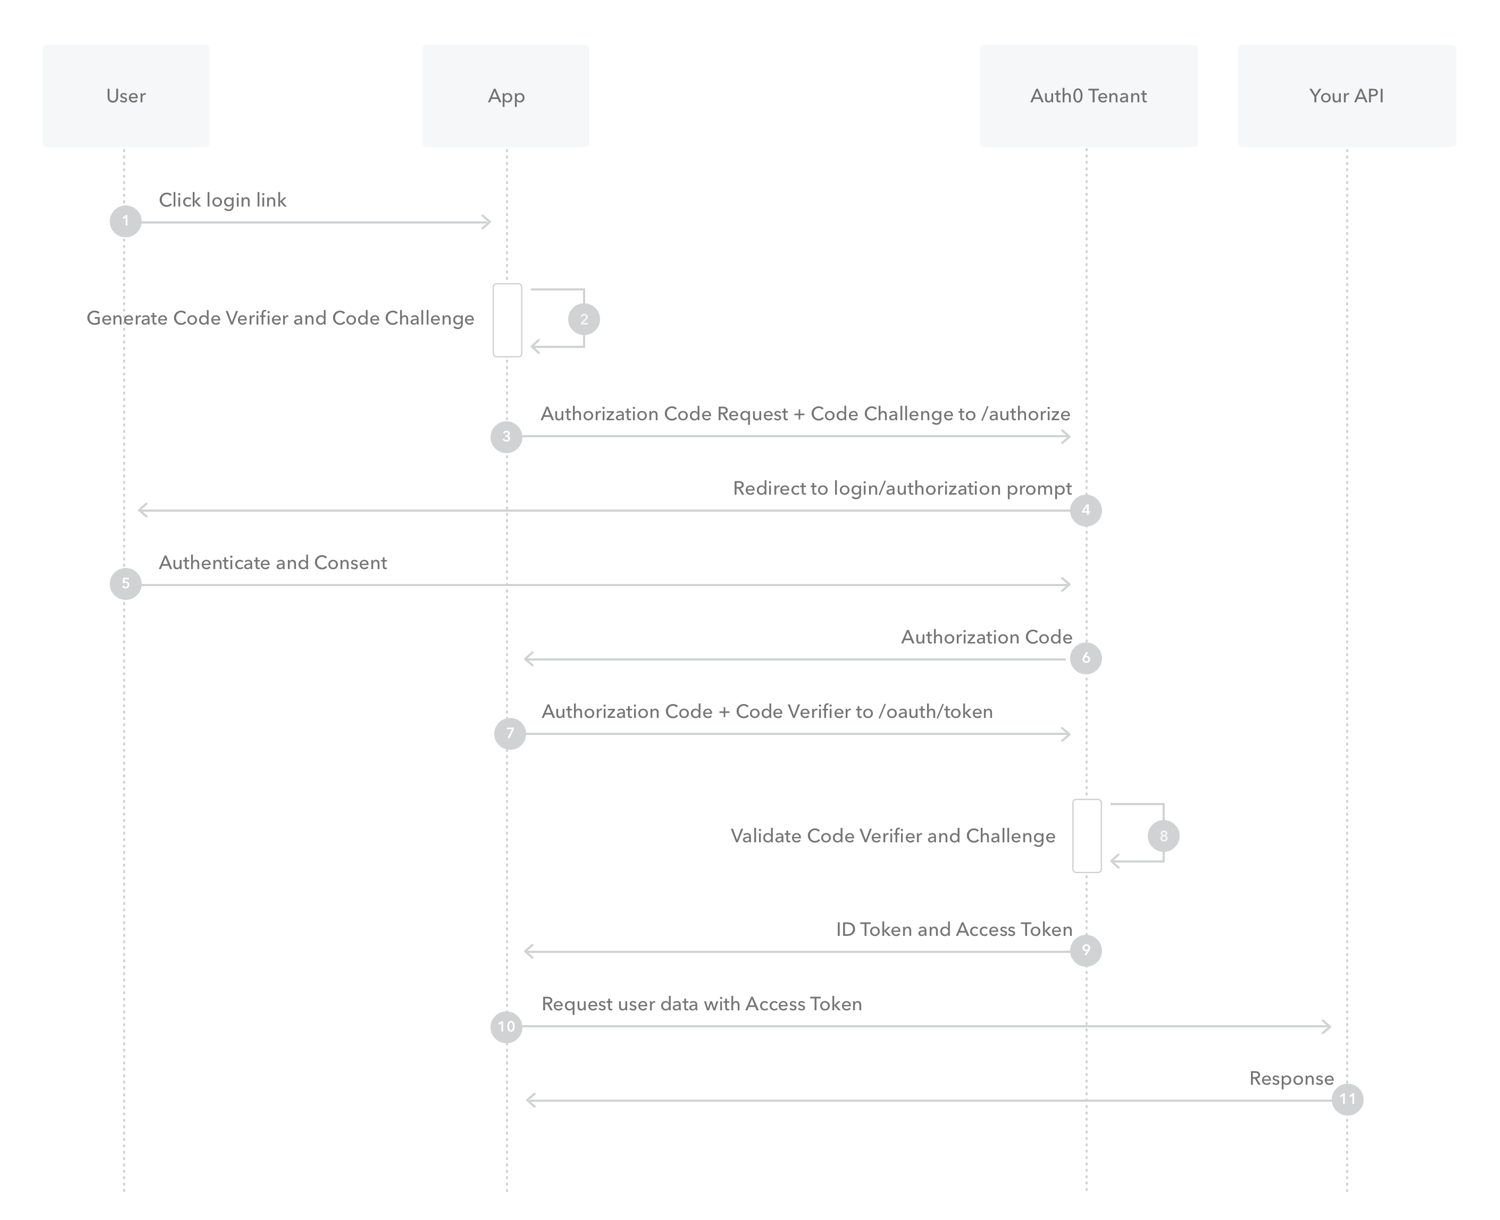
\includegraphics[width=0.85\textwidth]{figures/oauth}
    \caption{Authorization Code Flow with PKCE (source: Auth0 documentation~\cite{auth0PKCE})}
    \label{fig:oauth-flow}
\end{figure}

The IAM module exposes the public keys used for token verification via a JWKS endpoint,
which the API module reads at startup to configure its own authentication filter.

\subsection{The API Module}

\texttt{api} is the core of the application. It is deployed as a WAR under
\texttt{/rest-api} and provides all of the business logic: workspace management,
membership and role administration, epics, tickets, and their associated comments.

Its structure evolved significantly throughout the internship because the project followed
an agile/Scrum approach --- features were added, endpoint contracts revised, and the
authorization model refined sprint by sprint. The module is organized around resource
packages, each containing the endpoint class, DTO definitions, and the specific fetch,
create, update, and delete operations for a given entity (e.g.,
\texttt{EpicEndpoint}, \texttt{TicketEndpoint}, \texttt{MembershipEndpoint}).

Every protected endpoint passes through two Jakarta interceptors before reaching
business logic: an \textbf{authentication filter} that validates the JWT and sets the
caller's identity into a \texttt{ThreadLocal}, and a \textbf{workspace policy
enforcement point} that applies the ABAC rules defined in the core module.

\section{Frontend Architecture: The MVP Pattern}

The frontend is a pure vanilla JavaScript SPA. No framework, no npm dependencies at
runtime --- just ES modules served as static files. The company's constraint on external
JavaScript dependencies was non-negotiable, which meant the usual React or Vue abstractions
were off the table from the start.

In their place, Canny Vision has developed its own lightweight rendering engine built
around the \textbf{Model--View--Presenter (MVP)} pattern~\cite{fowlerMVP}. Getting to
grips with this pattern took a non-trivial amount of time, because it looks familiar on
the surface but enforces a stricter separation than most frontend developers are used to.

\begin{figure}[H]
    \centering
    \includegraphics[width=0.7\textwidth]{figures/mvpArchitecture}
    \caption{MVP architecture of the Canny Vision frontend engine}
    \label{fig:mvp}
\end{figure}

The engine is implemented in \texttt{scripts/mvp.js} and exposes three base classes:

\begin{itemize}
    \item \textbf{Model} extends \texttt{Observable} and is responsible for all API
          communication via a \texttt{callAPI} method. It maintains an internal LRU cache
          with configurable TTL and ETag support, so repeated GET requests do not always
          hit the network.
    \item \textbf{View} extends \texttt{Observable} and owns the DOM. It declares data
          bindings through a \texttt{defineBindings} method and applies them declaratively
          via \texttt{data-bind} attributes, supporting two-way binding for form inputs
          and one-way binding for display elements.
    \item \textbf{Presenter} wires the Model and View together. It registers as an observer
          on both, reacting to state changes from the model and intent events from the view.
\end{itemize}

The \texttt{Broker} class underpins the whole engine: it is a singleton publish/subscribe
bus that decouples the three layers so that neither the model nor the view holds a direct
reference to the other.

\section{Implementation Phases}

\subsection{Phase 0: Discovery and Infrastructure}

The first two weeks were deliberately not spent writing application features. They were
spent reading the existing IAM codebase, running WildFly, understanding how the existing
frontend starter kit was structured, and getting TLS to work end to end. The goal at the
end of this phase was a single, verifiable milestone: a browser sign-in button that
completed the full PKCE flow and landed back on the frontend with a valid JWT in
session storage.

\subsection{Phase 1: End-to-End Authentication}

Once the infrastructure was understood, the first real implementation task was to wire
three things together: the IAM module, a minimal API deployment (a sample Jakarta EE
project used as a scaffold), and the frontend starter kit. The sign-in flow had to work
end to end --- redirect to the IAM's \texttt{/authorize} endpoint, PKCE challenge and
verifier exchange, token returned to the frontend, and the access token attached to
subsequent API requests via the \texttt{Authorization: Bearer} header.

The client-side OAuth 2.0 logic lives in \texttt{scripts/iam.js}. It handles PKCE
code generation using the Web Crypto API, manages the redirect, exchanges the
authorization code for tokens at the \texttt{/oauth/token} endpoint, and stores the
result in session storage. It also handles token refresh on a background interval and
exposes a \texttt{checkSession} helper used by every page on load.

\subsection{Phase 2: Iterative API Development}

With authentication working, the focus shifted to the API module. Features were built
incrementally across Scrum sprints: workspace CRUD, membership management with role
assignment, the epic hierarchy, ticket management with assignment and status tracking,
and finally the comment system. At each step the ABAC policy was extended to cover the
new resources.

The endpoint contract changed multiple times as the team's understanding of the domain
deepened. The DTO structure, the role permissions matrix, the handling of workspace-scoped
identity (the membership token issued by the IAM alongside the access token) --- all of
these were refined through discussion and iteration rather than designed upfront in full.

\section{Chapter Conclusion}

Setting up the environment consumed more calendar time than anticipated, primarily because
WildFly and TLS-related issues required careful investigation rather than quick fixes.
That investment paid off: once the infrastructure was stable, the iterative feature
development proceeded smoothly, with each sprint delivering a functional increment. The
following chapter presents the results of that work through test scenarios, functional
walkthroughs, and a documented investigation into the most significant technical problem
encountered during integration.

% ============================================================
% RAW NOTES — kept for reference, not included in output
% ============================================================
% the first 2 week at canny vision were solely to understand the existing infrastructure
% I switched my os version from windows to linux to use wildfly effectively and set up the server
% talk about the stenghts of wildfly and how it's not your everyday server and how hard is it to set it up
% you can talk about how I spent 3 days trying to solve a problem where the server didn't allow cors request from the frontend to the api
% and how finally the problem was that the certficate used was created by sudo (sudo user) and when I set it up I used normal user
% ->so there was a mix in the certfifs :
% You were using mkcert to secure your local environment (iam.localhost). Even though you successfully imported the certificates into the Oracle JDK cacerts file using keytool, your Java code continued to throw SSLHandshakeException.
%
% (please read /middleware/core/configs to understand more)
% even though I didn't develop myslef the IAM module, understanding it was not an easy task
%
% the official documentation link to be included : https://auth0.com/docs/get-started/authentication-and-authorization-flow/authorization-code-flow-with-pkce
% I added on the figures folder an image figures/oauth that explain the flow of the authentication and authorization process in the system
%
% so my first task was to have a connecting iam module , api module (just old examlpe project) and frontend (just a starter kit with an mvp page example)
% and have a working sign -in flow
% I spent a hell of time understanding how the mvp patter work
% (I will provide in figures an image showing the architecure of mvp)
% (read from frontend/scripts/mvp.js to understand more)
% and read /frontend/scripts/iam.js to see how the iam connects to the frontned
%
% after getting the grasp of how everything works
% I started to implement the api module which is the core of the system
% and which its architectuee has changed many times during the internship since we worked in agile/scrum
% and kept on adding features and improving the design as we went along
%
% please talk about the folder strcuture of the middleware :
% how I used maven pom.xml to manage dependencies and build the project
% with three main modules : core, api and iam
% (read the folder middleware to understand more about the structure and the content of each module)
% talk about how core is the jar that contains all the common code and utilities that are shared between the api and iam modules
% and how the api module contains the business logic and the REST endpoints
% and how the iam module contains the authentication and authorization logic
%
% dear claude please take note that I am just throwing ideas ; and decide yourself the best order of the content

    \chapter{Analysis, Testing, and Performance Evaluation}

\section{Introduction}
This chapter presents the final realization through test scenarios, execution results, and performance analysis.

\section{Test Strategy}
Describe the testing approach and scope:
\begin{itemize}
    \item functional tests,
    \item integration tests,
    \item security and error-handling tests,
    \item performance-related checks.
\end{itemize}

\section{Test Scenarios and Results}
For each scenario, include:
\begin{itemize}
    \item objective,
    \item preconditions,
    \item execution steps,
    \item screenshots,
    \item observed results.
\end{itemize}

\section{Performance Metrics}
Present measurable indicators relevant to your context (QoS-oriented where applicable), such as:
\begin{itemize}
    \item response time and throughput,
    \item failure or error rates,
    \item resource usage,
    \item connection reliability,
    \item security-related indicators.
\end{itemize}

\section{Results Analysis}
Interpret the results and discuss whether objectives were achieved.

\section{Problems Encountered, Solutions, and Perspectives}
Conclude the chapter by summarizing:
\begin{itemize}
    \item key problems encountered,
    \item applied or proposed solutions,
    \item future improvement opportunities.
\end{itemize}





-- read /middleware/api/src/main/java/vision/canny/api/security/interceptors/AuthenticationFilter
(ai generated - to be simplified)
Concurrency Bug in JWT Authentication Filter — Investigation & Resolution
1. Problem Discovery
During the integration phase between the frontend application and the backend REST API deployed on WildFly, an intermittent and seemingly random authentication failure was observed. Certain API requests would return HTTP 403 Forbidden responses with the message "Access denied: subject has no membership in this workspace", despite the user being a legitimate member of the workspace in question. What made this particularly confusing was the non-deterministic nature of the failures — the same endpoint, called with the same token, would succeed on some invocations and fail on others, with no apparent pattern.

2. Initial Hypothesis: Frontend Issue
The first suspicion fell on the frontend. The natural assumption was that the JWT access token was either missing from some requests, malformed, or not being attached to the Authorization header correctly.

To verify this, logging was added to the authentication filter to print the full token value on every incoming request:


logger.info("****************** token is *******  " + token + "||| end of token");
The server logs confirmed that every failing request carried a valid, well-formed token — identical to the one used in successful requests. The frontend was not the problem.

3. Isolating with Postman
The next step was to reproduce the failure in a controlled environment using Postman. Every single request made through Postman succeeded without exception, even when repeated dozens of times against the same endpoints that were failing from the frontend.

This was a critical observation. It meant the bug was not in:

The token itself
The token validation logic in isolation
The database membership records
The business logic of the endpoint
The key difference between Postman and the frontend was that Postman sends requests sequentially, one at a time, while the frontend issues multiple parallel requests — fetching workspace data, user information, tickets, and other resources simultaneously upon page load.

This pointed directly toward a concurrency problem.

4. Log Analysis
Examining the WildFly server logs more carefully revealed the smoking gun. Two requests arriving at the exact same millisecond were being processed on two different threads:


2026-05-13 09:52:10,176 INFO [...AuthenticationFilter] (default task-18) *** token is *** eyJ0eXAi...
2026-05-13 09:52:10,176 INFO [...AuthenticationFilter] (default task-25) *** token is *** eyJ0eXAi...

2026-05-13 09:52:10,320 INFO [...WorkspacePolicyEnforcementPoint] (default task-18) ...developer
2026-05-13 09:52:10,320 INFO [...WorkspacePolicyEnforcementPoint] (default task-25) ...null

2026-05-13 09:52:10,330 WARNING [...] (default task-25) PIP — Subject 'null' has no membership in workspace 3
Both threads processed the same valid token at the same timestamp, yet one (task-18) correctly extracted the identity "developer", while the other (task-25) produced null. Since both tokens were identical and valid, the failure had to be happening inside the authentication filter itself during concurrent execution.

5. Root Cause Analysis
Bug 1 — Non-Thread-Safe Static Signature Instance (Critical)
The AuthenticationFilter class held a static field for the cryptographic Signature object used to verify JWT signatures:


private final static Signature signatureAlgorithm; // shared across ALL threads
In Java, static fields belong to the class, not to any instance — meaning one single Signature object was shared across every concurrent request.

java.security.Signature is a stateful, sequential object. Its correct usage follows a strict three-step protocol:


1. initVerify(publicKey)          — initialize with the key
2. update(dataBytes)              — feed in the data to verify
3. boolean result = verify(sig)   — perform the check
Under concurrent load, two threads executing these steps on the same shared object interleave in unpredictable ways:

Thread task-18	Thread task-25
initVerify(key)	
initVerify(key) ← resets object state
update(data)	
verify(...) ← operates on corrupted state → returns false	
When verify() returned false, the authentication filter treated the request as if the signature was invalid and skipped the entire identity-setting block — never calling IdentityUtility.iAm(sub). The ThreadLocal storing the username remained null from a previous (or never-initialized) state. The downstream interceptor then read null as the subject identity, resulting in the membership check failing with a 403.

Bug 2 — Non-Thread-Safe HashMap Cache
A secondary concurrency hazard was identified in the public key cache:


private final static Map<String, PublicKey> CACHE = new HashMap<>();
HashMap is not thread-safe. Concurrent reads and writes — particularly during cache population when a new kid (key ID) is encountered — can corrupt the map's internal structure, leading to lost entries, infinite loops, or exceptions. While this was less likely to manifest visibly, it represented a latent race condition in the same code path.

6. The Fix
Fix 1 — Per-Request Signature Instance
The static Signature field was removed entirely. Instead, a new Signature instance is created locally inside the filter method for each request:


// Before — one shared instance, not thread-safe
private final static Signature signatureAlgorithm = Signature.getInstance(curve);

// After — fresh instance per request, fully isolated
var signatureAlgorithm = Signature.getInstance(curve); // inside filter()
Each thread now has its own independent Signature object. There is no shared mutable state, and concurrent requests cannot interfere with each other's verification process. The instantiation cost is negligible.

Fix 2 — ConcurrentHashMap for the Key Cache
The HashMap was replaced with ConcurrentHashMap, the standard Java library's thread-safe alternative:


// Before
private final static Map<String, PublicKey> CACHE = new HashMap<>();

// After
private final static Map<String, PublicKey> CACHE = new ConcurrentHashMap<>();
ConcurrentHashMap provides safe concurrent access without requiring explicit synchronization, making it the appropriate choice for a shared, application-scoped cache.

7. Lessons Learned
This bug illustrates a class of defects that is particularly insidious in server-side Java development:

Static mutable state in a multi-threaded environment is a concurrency hazard. In a Jakarta EE / WildFly deployment, request-handling classes are instantiated once and reused across threads. Any static field holding a stateful, non-thread-safe object becomes a shared resource contended by all concurrent requests.

The failure was especially difficult to detect because:

It was non-deterministic — it only manifested when two requests arrived within the same millisecond
It was not reproducible in isolation — sequential testing tools like Postman never triggered the race condition
The symptom (null identity → 403) appeared in a completely different layer (the ABAC interceptor) from the actual cause (the authentication filter), making the stack trace misleading
The debugging methodology that revealed the root cause was the combination of:

Confirming the token was present (eliminating the frontend)
Confirming the bug never reproduced under sequential load (pointing to concurrency)
Reading timestamps in the server logs precisely (confirming two threads processed the same token simultaneously with divergent outcomes)
    \chapter*{General Conclusion}
\addcontentsline{toc}{chapter}{General Conclusion}

The general conclusion must address all of the following points, as required by the SUP'COM PFE guide:
\begin{itemize}
    \item \textbf{Problem recall} --- briefly restate the problem and the objectives that were set at the outset.
    \item \textbf{Summary of work} --- synthesize the main tasks carried out across each chapter.
    \item \textbf{Key results and contributions} --- highlight the most significant outcomes and the student's own contributions.
    \item \textbf{Critical assessment} --- discuss limitations, difficulties encountered, and lessons learned.
    \item \textbf{Perspectives} --- propose concrete directions for continuing or extending the work.
\end{itemize}


    \begin{appendices}
        \chapter{Appendix A: Supplementary Technical Artifacts}

Use this appendix for supporting material such as:
\begin{itemize}
	\item additional architecture diagrams,
	\item API endpoint extracts,
	\item database schema snapshots,
	\item extra implementation screenshots.
\end{itemize}

        \chapter{Appendix B: Testing and Validation Evidence}

Use this appendix for extended validation material such as:
\begin{itemize}
	\item full test case tables,
	\item raw logs and benchmark outputs,
	\item error traces and troubleshooting records,
	\item supplementary result graphs.
\end{itemize}

    \end{appendices}

    \bibliography{references}

\end{document}